\chapter{Common Lifetime Patterns}
\index{Lifetime Patterns}
It would be great if programmers could be in charge only of hooking together and
populating their data structures, leaving the \jre responsible for the details of
object allocation and reclamation. The Java runtime does indeed help manage some
aspects of these management tasks, but leaves a good deal of work in your hands.
In Java, you needn't explicitly free objects, and in that way a managed language
is a big step up from a language like C. However, the ultimate promise of
automatic memory management, that you can create objects without regard for messy
details of storage management, doesn't play out ideally in practice. Unless you
are careful, your program will suffer from bugs such as memory leaks, and suffer
from poor performance. Furthermore, if your objects don't easily fit into the
limits of a single Java process, and you need to manage, explicitly, shuttling
them in and out of the Java heap.

Unfortunately, then, it is necessary to plan out the lifetime of your objects.
Your application needs some objects to live forever and it needs the rest to die
a timely death. This task of managing object lifetime is made simpler by the
fact that there aren't innumerable ways in which objects live and die. For the most part, your objects
will fall into one of five common patterns of lifetime.
\autoref{tab:five-lifetimes} summarizes these five important patterns.
% This often requires careful design on your part, both to avoid bugs and so that
% your application performs well in the case when not everything fits into the
% Java heap.

%The trickier aspects of memory management, summarized in
%\autoref{tab:tricky-memory-management}, are discussed in greater detail in
%later chapters.

\begin{table}
\centering
	\begin{tabular}{lp{0.30\textwidth}p{0.35\textwidth}}
	\toprule  & Lifetime Property & Example \\ \cmidrule(r){2-2} \cmidrule(l){3-3}
	\autoref{temporary-lifetime}  & {Temporary} & new
	parser for every date
	\\
	\autoref{forever-lifetime} & {Needed Forever} & product catalog
	\\
	\autoref{correlated-lifetime-1} & {Correlated with Object}
	& object annotations
	\\
	\autoref{correlated-lifetime-2} & {Correlated with Phase} &
	DOM used only for parsing
	\\
	\autoref{deferred-deletion} & {Deferred Deletion} &
	session state \\
%period\\ scoped to a phase/request\\
%correlated with an object (annotations)\\
%correlated with need}\\ \hline
%reusable & maybe i'll need it later \\ \hline
	\bottomrule
	\end{tabular}
	\caption{Five important categories of object lifetime.}
	\label{tab:five-lifetimes}
\end{table}

\section{Examples from a Server Application}

Configuring memory settings is an iterative process. It usually involves a
fair amount of trial and error, as one tunes the various knobs to balance memory
consumption and application performance. These knobs affect things like the size of the Java
heap, how many entries a cache should hold, and the timeout value for these
caches. This is usually a process of black box tuning: twist a knob, and see
how overall performance changes. In addition to being hit
and miss, it is also quite prone to bugs. If you set the size of a cache too
high, you risk poor performance due to excessive garbage collection, and even
possibly process failures, due to running out of heap space.

Tuning memory consumption in long-running applications, such as servers or
integrated development environments, is a particularly thorny issue. Improperly
managing memory in a short-running application may not be the end of the world.
In an application that runs more or less forever, mistakes can pile up over time.
In addition, they synthesize information from a diverse array of sources, each
with its own performance trade-offs. As such, caching plays a large role in these
applications. Consider an example from a server aplication.

\begin{example}{Object Lifetimes in a Server Application}
A web application commerce server preloads catalog data into memory to allow for
quick access to this commonly used data. It also maintains data for users as they
interact with the system, browsing and buying products. Finally, it 
caches the response data that comes from a remote service provider that charges
per request. How does Java heap consumption vary over time? Which heap size
fluctuations indicate a problem, and which are expected behavior?
\end{example}

\begin{figure}
	\centering
	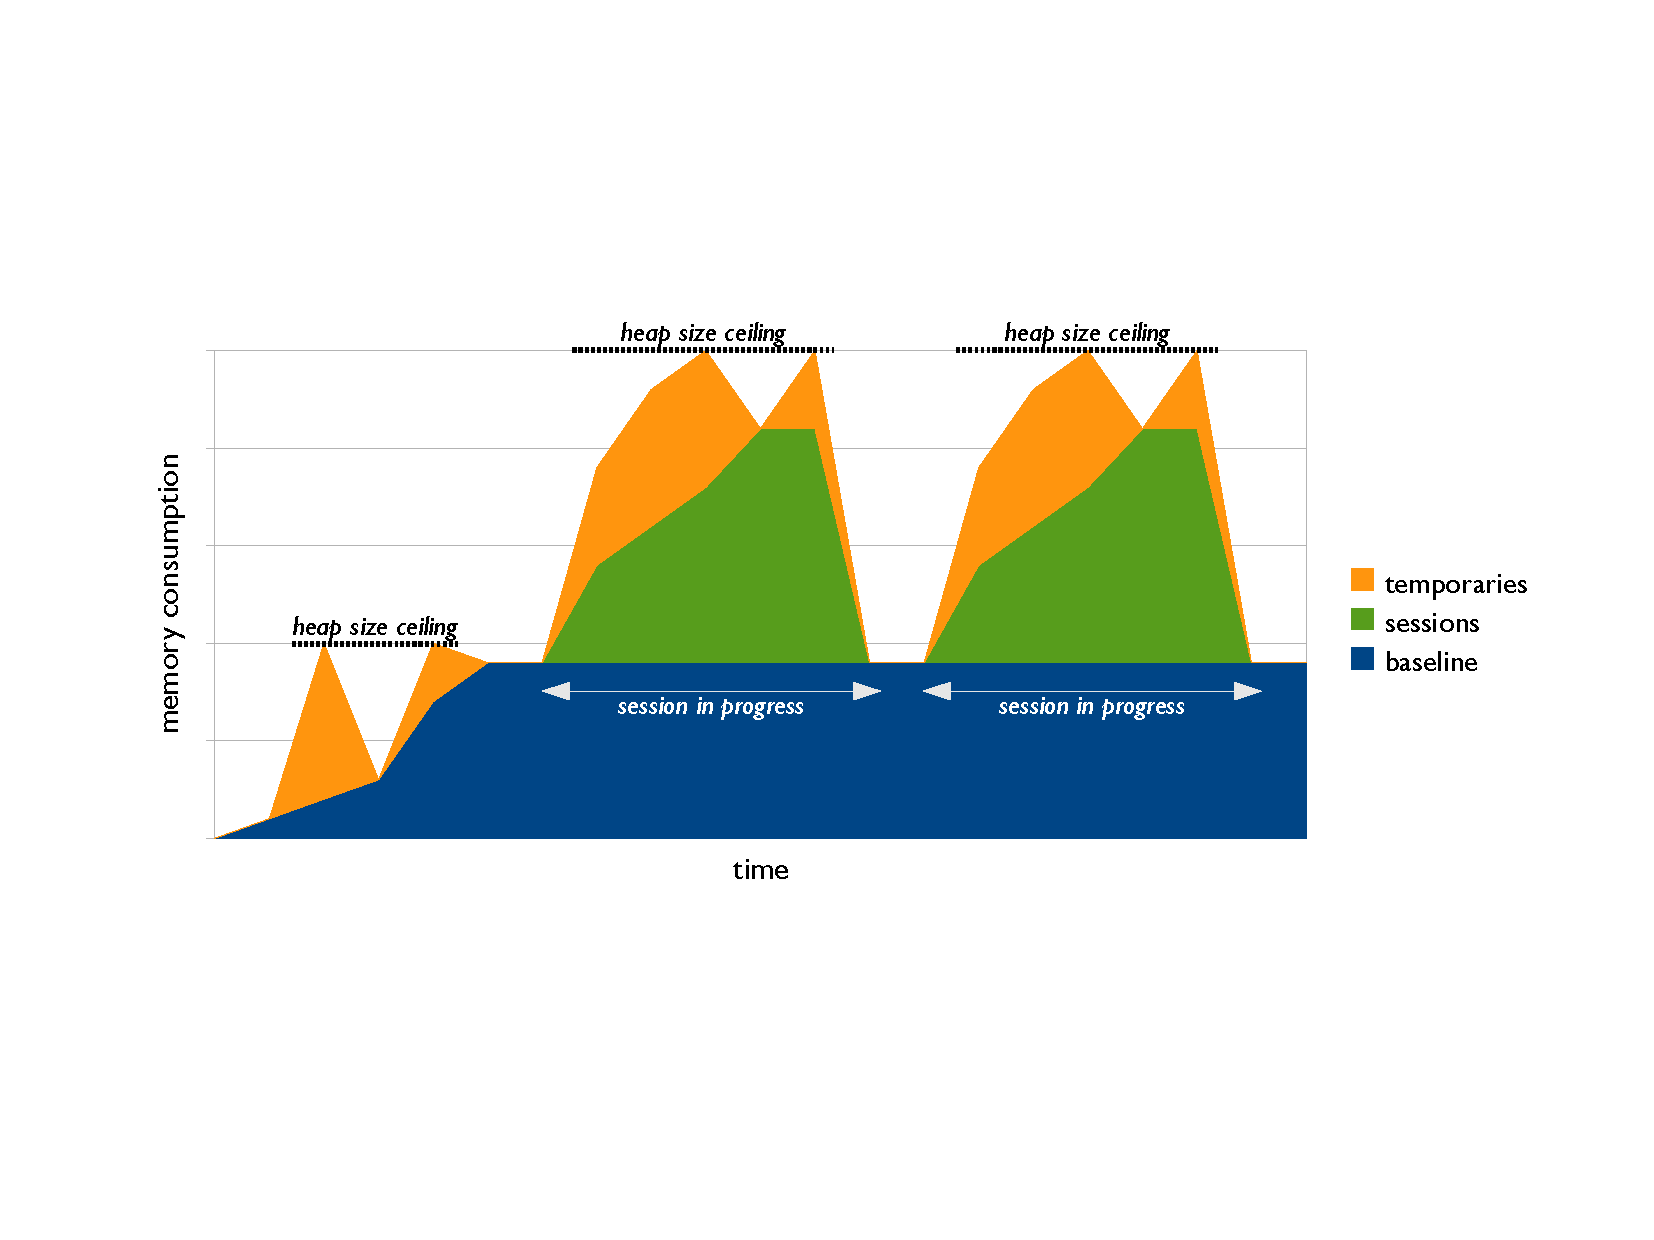
\includegraphics[width=\textwidth]{Figures/lifetime/timeline-base-session-temps}
	\caption{Memory consumption, over time, typical of a web application server.}
	\label{fig:timeline-base-session-temps}
\end{figure}

The heap consumption of this application will fluctuate over time. A timeline
view expected memory consumption helps to illustrate the five main kinds of
object lifetime. It visualizes memory during the lulls and peaks of activity, as
requests are processed and when sessions time out, and as the server starts up.
 \autoref{fig:timeline-base-session-temps} shows an example timeline
for a server that, as it starts up begins to load catalog data into the Java heap.
Then, it responds to one request at a time. The total height of the area under
the curves represents the memory consumption at that point in time. 
In this example, as the server starts up, it begins to load catalog data into
the heap. This data will be used for the entire duration of the server process.
\index{Objects That Live Forever}
The Java objects that represent this catalog are objects that are needed
forever. In the timeline picture, this data is respresented by the lowest area,
labeled \emph{baseline}. Notice how it ramps up quickly, and then, after the
server has reached a ``warmed up'' state, memory consumption of this baseline
data evens out on a plateau for the remainder of the run.

\index{Session State}
After the server is warmed up, it begins to process client requests. Imagine
interacting with a commerce site. First you browse around for items of
interest. You may add items to your shopping cart. Eventually, you may
authenticate and complete a purchase. 
As you browse and buy, the server may be maintaining some
state, to remember aspects of what you have done so far. This
session state, at least the part of it stored in the Java heap, will go away
soon after your browsing session is complete. In the timeline figure, this
portion of memory is labeled \emph{sessions}. It ramps up while a session is in
progress, and then, in the example illustrated here, soon all of that session
memory should be reclaimed.

The catalog (baseline) data and session state are both examples of objects that
are expected to stick around for a while.
\index{Temporary Objects}
 In the course of preloading the cache
and responding to client requests, the server application will create a number
of objects that are only used for a very short period of time. They help to
faciliate the main operations of the server.
These temporary objects will be reclaimed by the \jres garbage collector in
relatively short order. The point at which an object is reclaimed depends on when the garbage collector
notices that it is reclaimable. Normally, the garbage collector will wait until
the heap is full, and then inspect the heap for the objects that are still
possibly in use. In this way, the area under the \emph{temporaries} curve has a
see-saw shape. As the temporaries pile up, waiting for the next garbage
collection, they contribute more and more to memory footprint. Normally, once
the \jre runs a garbage collection, these temporaries no longer in use will no
longer contribute to heap consumption.

In this way, temporary objects
\emph{fill up the headroom} in the heap.\index{Heap Headroom}. If there is a
large amount of heap space unused by the longer-lived objects, then the
temporaries can be reclaimed less often. This is a good thing, because a
garbage collection is an expensive proposition.
\index{Heap Size Settings} \index{Maximum Heap Size} \index{-Xmx}
When configuring your application, you may specify a maximum heap size. It
should certainly be larger than the baseline and session data. How much
larger than that? This choice directly affects the amount of \emph{headroom},
 that is the amount of space available for temporaries to pile up.

\begin{figure}
	\centering
	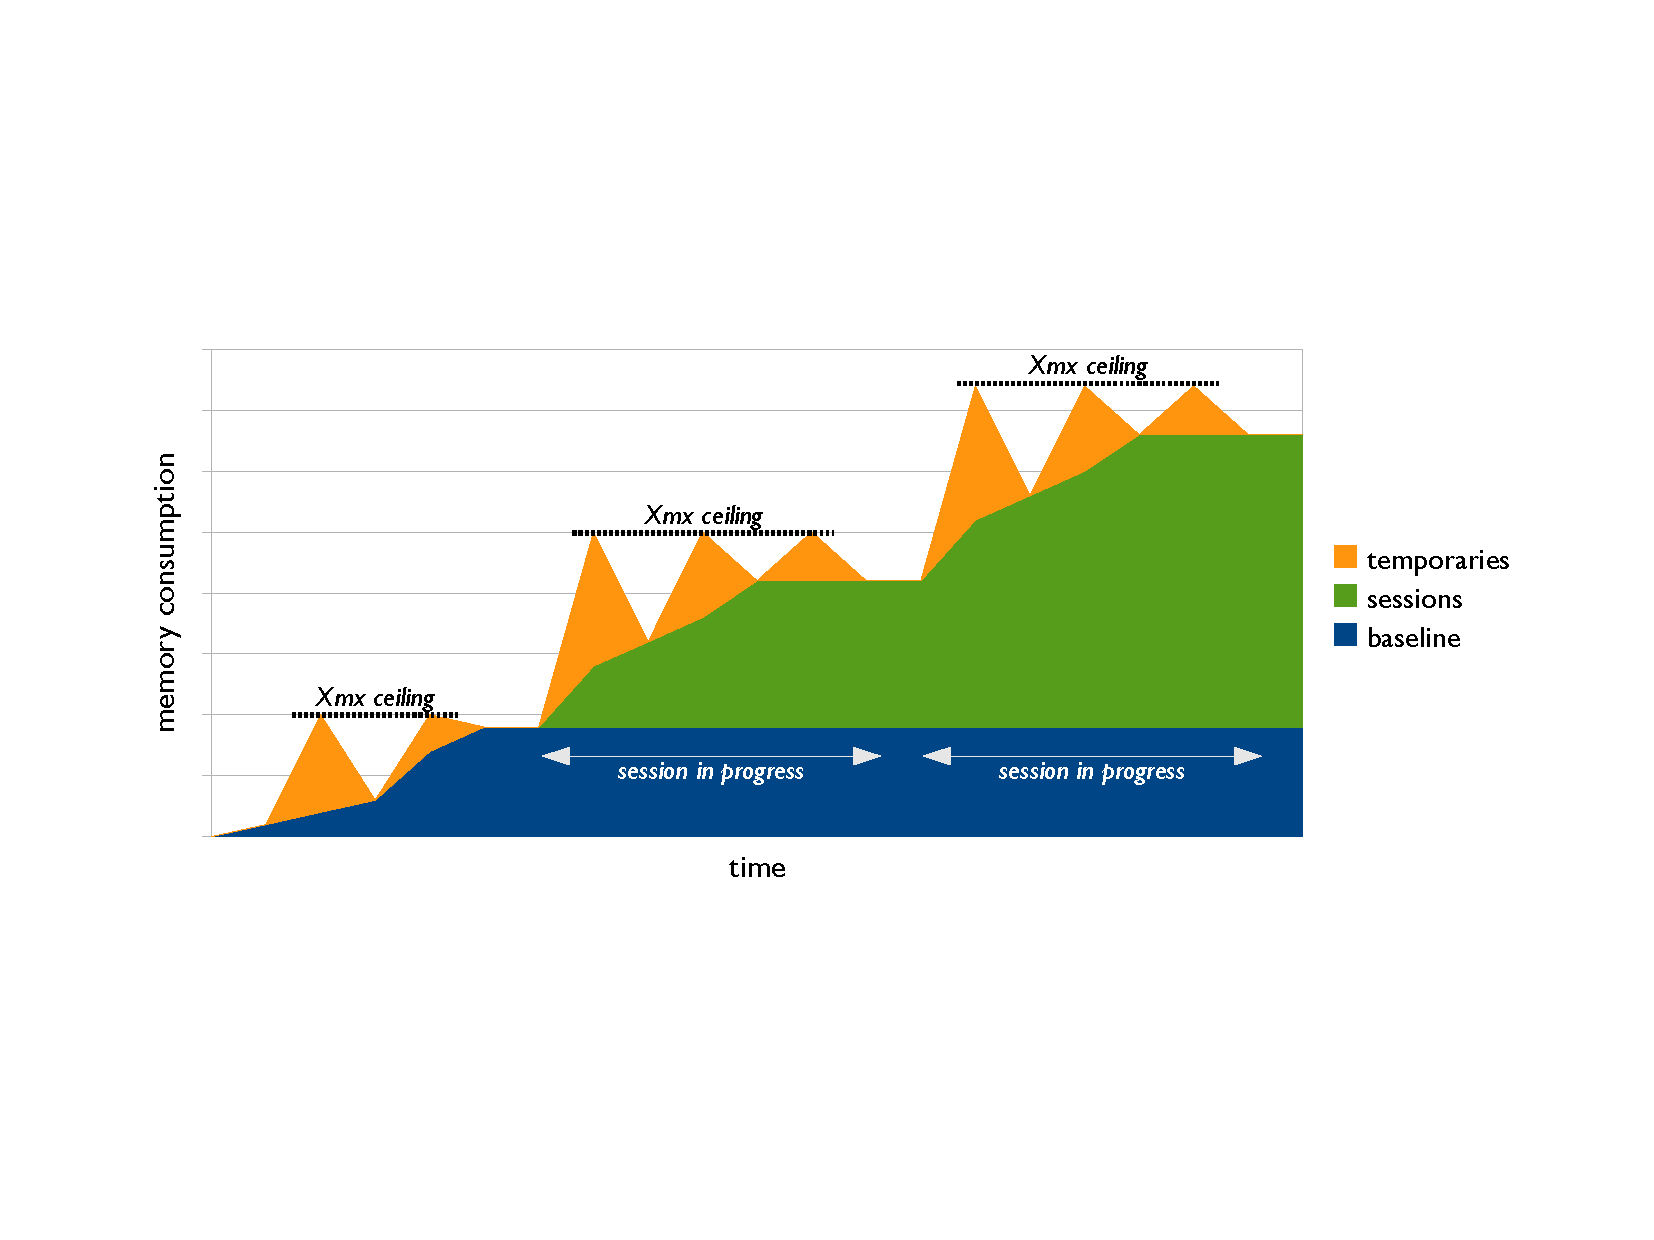
\includegraphics[width=\textwidth]{Figures/lifetime/timeline-base-session-temps-with-leak}
	\caption{If session state is not cleaned up
	properly, a memory leak is the result. This means more frequent garbage
	collections, and ever increasing heap size.}
	\label{fig:timeline-base-session-temps-with-leak}
\end{figure}

\index{Memory Leaks}
The catalog data should last forever, while the
session data lives for some bounded period of time. It is possible that session
state will live beyond the end of your session, but nonetheless it has a
lifetime that is bounded. If, due to an bug, part of this session state is not
reclaimed, the application will leak memory. Though it is supposed to have a bounded lifetime, it
\marginpar{\textbf{Memory Leaks} are still possible, even with
automatic garbage collection!} accidentally lives forever. In this
case, over time, the amount of heap required for the application to run will increase without bound.
\autoref{fig:timeline-base-session-temps-with-leak} illustrates this situation,
in the extreme case when all of session state leaks. Over time, the area under
the curve steps higher and higher.

%As you scan the timeline from left to right, memory consumption 
%it fetches catalog data from its database, and stores them in the Java heap. 

Finally, this example server caches data from some expensive third-party data
source. When caching data inside of Java objects, there is a fourth effect on
the timeline landscape. The
cached data must be configured properly to live long enough to be useful. It
also must not occupy so much of the heap so as to leave little headroom for
temporaries. \autoref{fig:timeline-base-session-temps-with-cache} shows an
example where the cache has probably been configured to occupy too much heap
space. Observe how, compared to the other timeline figures, there is little
headroom for temporaries. In this case, the result is more frequent garbage
collections. If the cache were sized to occupy an even greater amount of heap
space, it is possible that there would no longer be room to fit session data.
The result in this case would be failures in client requests. So, as you can
see, sizing caches is important. As discussed later, it is very tricky to
properly size caches, and is something best left in the hands of the \jre.

\begin{figure}
	\centering
	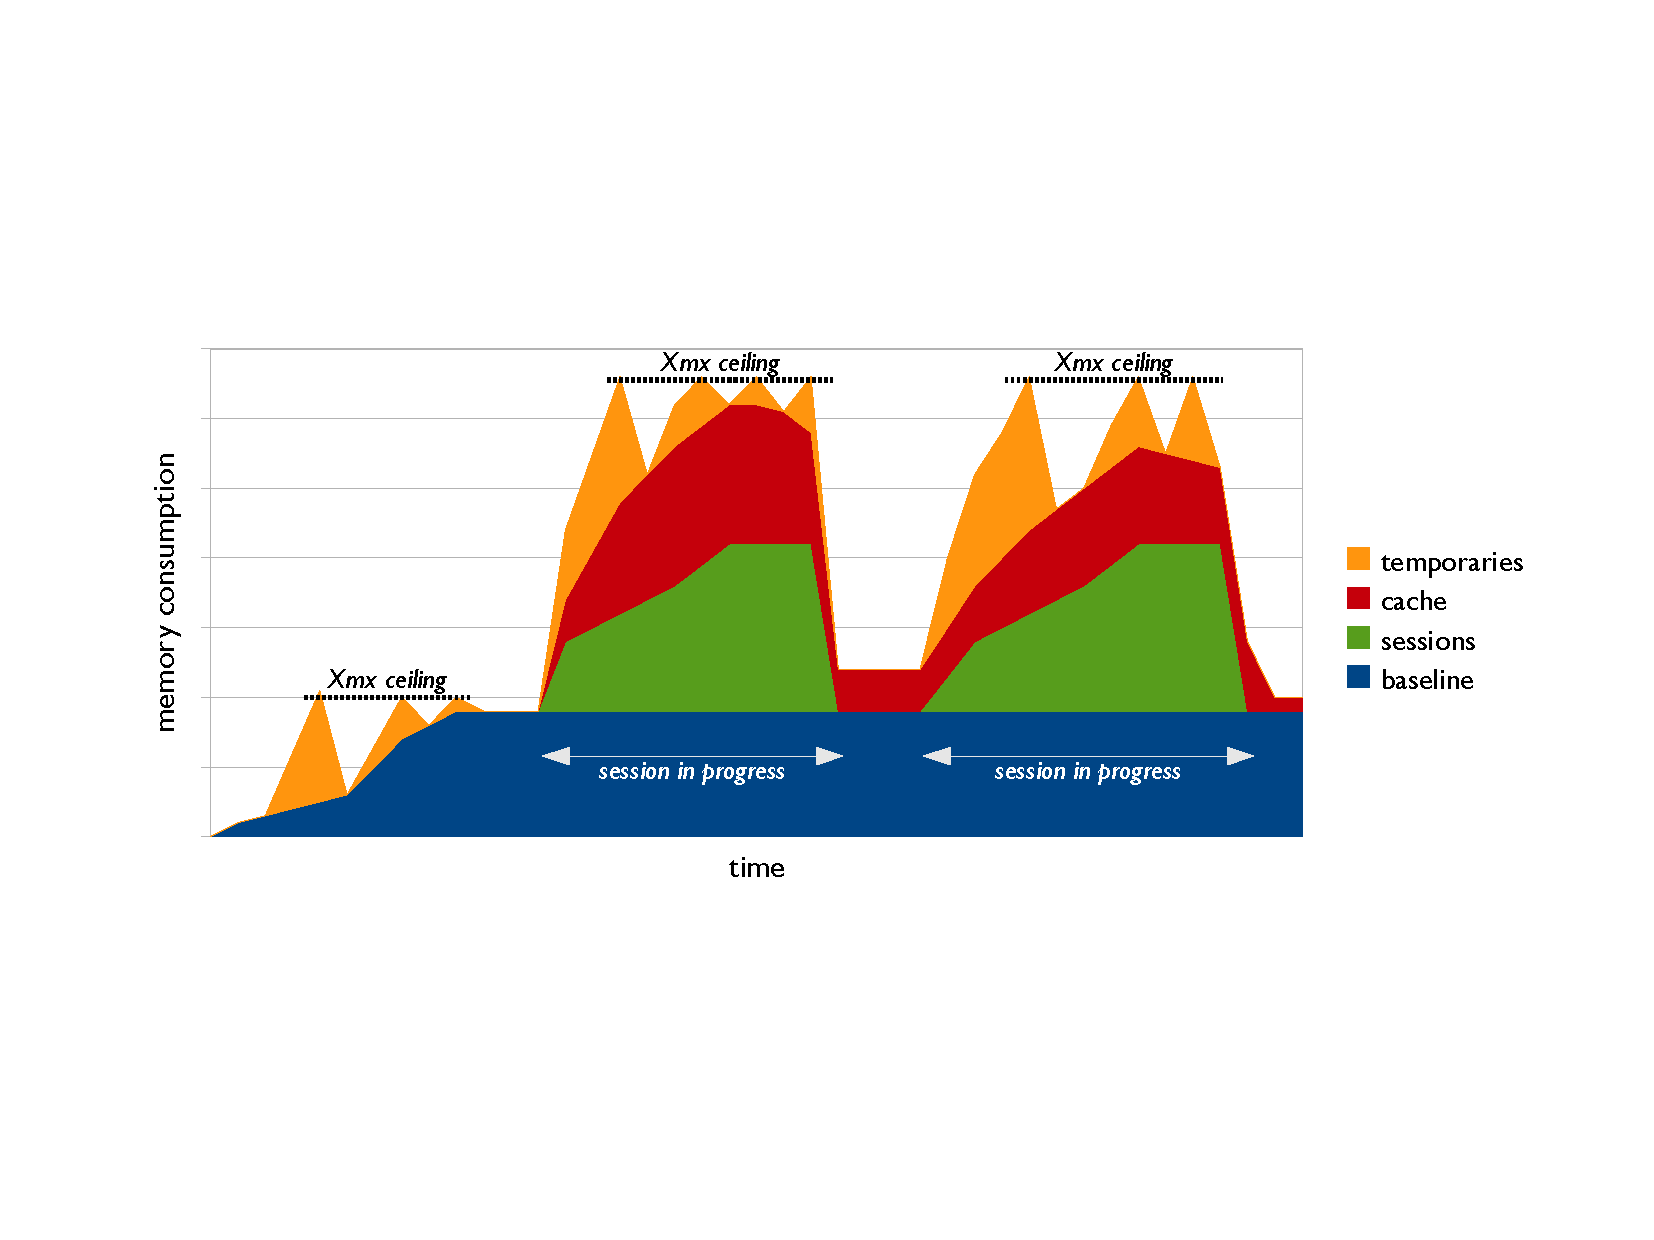
\includegraphics[width=\textwidth]{Figures/lifetime/timeline-base-session-temps-with-cache}
	\caption{When a cache is in use, this leaves less headroom for temporary
	object allocation, often resulting in more frequent garbage collections.}
	\label{fig:timeline-base-session-temps-with-cache}
\end{figure}

% introduced by example in this chapter, and
%Many objects are either temporaries or needed for
%the entire run of your application. Sometimes you create objects whose lifetime
%is correlated with other objects or that should go away when a method
%invocation completes. Sometimes you need to manage objects hanging around
%longer than their current need, to avoid future recomputations or refetching
%of data in the case when it is needed in the near future. 

%\begin{table}
%\centering
	%\begin{tabular}{ll} \toprule
    %%%%	%& Things Java Doesn't Do Automatically \\ \cmidrule{2-2}
%    	\autoref{avoiding-lifetime-bugs} & {Avoiding Memory Leaks} \\
%    	\autoref{balance-time-and-space} & {Balancing Time and Space} \\
%    	\autoref{outisde-java-box} & {Supporting Massive Data Sets}  	\\
%        \bottomrule
%    \end{tabular}
%	\caption{The tricky aspects of memory management.}
%	\label{tab:tricky-memory-management}
%\end{table}

\section{Temporary Objects}
\label{temporary-lifetime}

If your application is like most Java applications, it creates a large number of
temporary objects. They hold data that will only be used for a very short
interval of time. It is often the case that the objects in these transient data
structures are only ever referenced by local variables. For example, this is the
case when you populate a \class{StringBuffer}, turn it into a \class{String}, and
then ultimately (and only) print the string to a log file. The point at which all
of these objects, the strings and character arrays, are no longer used is only
shortly after they are constructed. These objects serve as transient homes for
your data, as it makes its way through the frameworks and libraries you depend
on. Temporaries are often necessary to bridge separately developed code and
enable code reuse: as long as you can convert your data layout into a form that
an API requires, then you can reuse the functionality it provides.

In many cases, you need do nothing special to manage the temporary objects your
application creates. After all, generational garbage collectors these days do a
very good job digesting a large volume of temporary objects. In a generational
garbage collector, the \jre places temporary objects in a separate heap, and
thus it need only process the newly created objects during its routine scan.

Unfortunately, in Java it is pretty easy to create a high volume of temporary
objects. Say your application 
fills up the temporary heap ever second. In this case, based on the common
speeds of garbage collectors, your application could easily spend over 20\% of its time
collecting garbage.
Is it difficult to fill up the temporary heap once per second? Typical
temporary heap sizes run around 128 megabytes. Say your application is a serves
a peak of 1000 requests per second, and creates objects of around 50 bytes each.
If it creates around 2500 temporaries per request, then this application will
spend 20\% of its time collecting garbage.


%A great many of these
%temporary structures serve the role of a kind of lubricant, making it easy for
%you to write code that ties together the separately written parts of your code
%base and reuses standard libraries as much as possible. Often, these are
%objects that are not a fundamental necessity of what you're trying to
%accomplish. If
%you had the freedom to code highly specialized implementations of the important
%cases, from scratch, many of these temporary structures would be unnecessary.

\begin{example}{How Easy it is to Create Lots of Temporary Objects}
A common example of temporaries is parsing
and manipulating data coming from the outside world. Identify the temporary
objects in the following code.
% to the wire?

\begin{shortlisting}%[float,caption=Code that constructs 8 temporary objects tohandle two dates.,label=TempExampleCode]
void main(String xy) {
	doWork(xy.substring(0,10), xy.substring(10));
}	
void doWork(String x, String y) {
	doRemoveProcedureCall(parse(x));
	doRemoveProcedureCall(parse(y));
}
Date parse(String string) {
	return new SimpleDataFormat().parse(string, new ParsePosition(0));
}
void doRemoteProcedureCall(Date date) {
	long timestamp = date.getTime();
	...
}
\end{shortlisting}
\end{example} 

This code starts in the \code{main} method by splitting the input string into two
substrings. So far, the code has created four objects (one \class{String} and one
character array per substring). Creating these substrings makes it easy to use
the \code{doWork} method, which takes two Strings as input. However, observe that
these four objects are not a necessary part of the computation. Indeed, these
substrings are eventually used only as input to the \class{SimpleDateFormat}
\code{parse} method, which has been nicely designed to allow you to avoid this
very problem. By passing a \class{ParsePosition}, one can parse substrings of a
string without having to create temporary strings (at the expense of creating
temporary \class{ParsePosition} objects!).



% correlated with need: as soon as last user goes away, remove his stuff 
% share common expressions to save space, but using strong references -> memory
% leak; plugins in eclipse go away when all views
% sharing pool 

% weak ref keys -> annotation
% weak ref values -> sharing pool

% soft ref values -> caching

% annotation by map lookup


\section{Objects Needed Forever}
\label{forever-lifetime}

A \class{SimpleDateFormat} object in the previous example was created in every
loop iteration, and never used again. An improvement would be to create and
use a single formatter for the remaining duration of the run. Though the Java 6
documentation does not say so explicitly, it is safe to reuse a single instance
of this object multiple times. You must be careful to remember that it is
not safe to do so in multiple threads. The next chapter will discuss remedies
to this problem. The updated code for the \code{parse} method would be:

\begin{shortlisting}
static final DateFormat fmt = new SimpleDateFormat();

Date parse(String string) {
	return fmt.parse(string, new ParsePosition(0));
}
\end{shortlisting} 

A \code{static} field of an object is one way that Java gives you to indicate
that you want an object to live forever.

\section{Objects with Correlated Lifetimes}

Many objects are needed for a very specific interval of time. This interval is
usually defined either by the lifetime of another object, or by the duration of
a method call. Once that other object is not needed, or once that method
returns, then these objects are also no longer needed. These are the two many
cases of objects with correlated lifetime.

\subsection{Objects that Live and Die Together}
\label{correlated-lifetime-1}

Normally, if you need to augment the state stored an object, you modify
the source code of some existing classes. For example, to add a secondary
mailing address to a \class{Person} object, you can add a field to that class, and update the
initialization and marshalling logic accordingly. Sometimes, you will find it
necessary to associate information with an object that is, for one reason or the
other, locked down.

\begin{example}{Annotations}
In order to debug a performance problem, you need to associate a timestamp with
another object. Unfortunately, you don't have access to the source code for
that object's class. Where do you keep the new information, and how can you
link the associated storage to the main objects without introducing memory
leaks?\index{Memory Leaks}
\end{example}

If you can't modify the class definition for that object, then you will have to
store the extra information elsewhere. These \emph{side annotations}\index{Side
Annotations} will be objects themselves, and you need to make sure that their
lifetimes are correlated with the main objects. When one dies, the other
should, too.

You could store the annotations in a map that is keyed by the
original object, say of type \class{T}:

\begin{shortlisting}
Map<T, Date> timestamps = new HashMap<T, Date>();

void addTimestamp(T t) {
	timestamps.put(t, new Date());
}
Date getTimestamp(T t) {
	return timestamps.get(t);
}
\end{shortlisting}

This solution will function correctly, but suffers from a \emph{memory
leak}\index{Memory Leak}. As the application runs, it will consume greater
amounts of Java heap, up until the point when the \jre runs out of heap space to
allocate any more objects. This solution leaks memory, because the
\code{timestamps} map introduces a reference to the main objects. When the
garbage collector scans the heap to see which objects are still alive, the
references in this map will be among those that keep the objects alive. The next
chapter discusses these issues in more detail. An improved solution would use the
\class{WeakHashMap} from the Java standard libraries. By replacing the
initialization of the \code{timestamps} map, we have the same functionality as
before, but no memory leak.

\begin{shortlisting}
Map<T, Date> timestamps = new WeakHashMap<T, Date>();
\end{shortlisting}

Note that this same situation can hold even if you are able to modify the class
definition. A common scenario requires annotations on only a subset of all
instances of a class. In this case, is it not worth paying the memory cost to
have the ability to annotate every single instance. Therefore, this is another
case where a solution of side annotations, stored in a \class{WeakHashMap},
shines.

\subsection{Objects that Live and Die with Program Phases}
\label{correlated-lifetime-2}

Similar to the way the lifetime of an object can be correlated with another
object, lifetimes are often correlated with method invocations. When a method
returns, objects correlated with it should go away. For temporary objects, this
is usually easy to ensure, since they are usually only referenced by stack
locations. For the medium-to-long running methods that implement the
core functionalities of the program, this correlation is harder to get right.

For example, if your application loads a log file from disk,
parses it, and then displays the results to the user, it has roughly three
phases for this activity. Most of the objects allocated in one phase are scoped to that
phase; they are needed to implement the logic of that phase, but not subsequent
phases. The phase that loads the log file is likely to maintain maps that
help to cross reference different parts of the log file. These are necessary
to facilitate parsing, but, once the log file has been loaded, these maps can be
discarded. In this way, these maps live and die with the first phase of this
example program. If they don't, because the machinery you have set up to
govern their lifetimes has bugs, then your application has a memory
leak\index{Memory Leaks}.

This lifetime scenario is also common if your application is an
server that handles web requests.

\begin{example}{Memory Leaks in an Application Server}
	A web application server handles servlet requests. How is it possible that
	objects allocated in one request would unintentionally survive beyond the end
	of the request?
\end{example} 
  
In server applications, most
objects created within the scope of a request should not survive the
request. Most of these \emph{request-scoped}
\index{Request-scoped Lifetime} objects are not used by the application after the
request has completed. In the absence of application or framework bugs, they will
be collected as soon as is convenient for the runtime. In this example, the
lifetime of objects during a request are \emph{correlated} with a method
invocation: when the servlet \class{doGet} or \class{doPut} (etc.) invocations
return, those correlated objects had better be garbage collectible.

\index{Memory Leaks: Why?}
There are many program bugs and configuration missteps that can lead to
problems. The general problem is that a reference to an object stays around
indefinitely, but becomes
\emph{forgotten}, and hence rendered unfindable by the normal application
logic. If this request-scoped data structure were only reachable from stack
locations, you would be fine. Therefore, a request-scoped object will leak only
when there exist references from some data structure that lives forever. Here
are some common ways that this happens.

\begin{itemize}
  \item Registrars, where objects are registered as listeners to some service,
  but not deregistered at the end of a request.
  \item Doubly-indexed registrars. Here the outer map provides a key to index
  into the inner map. A leak occurs when the outer key is mistakenly
  overwritten mid-request. This can happen if the namespace of keys isn't
  canonical and two development groups use keys that collide. It can also
  happen if there is a mistaken notion, between two development groups, of who
  owns respnsibility of populating this registrar.
  \item Misimplemented hashcode or equals, which foils the retrieval of an
  object from a hash-based collection. If developers checked the return value of
  the \code{remove} method, which for the standard collections would indicate a failure to remove, then
  this bug could be easily detected early; but developers tend not to do this.
\end{itemize}

The next chapter goes into greater detail on how to avoid these kinds of
errors. (Some other) chapter describes tooling that can help you detect and
fix the bugs that make it into your finished application.


%\subsection{Correlated with Need} % do we need this? isn't session state a
% deferred deletion policy?
%\label{correlated-lifetime-3}

\section{Objects with Deferred Deletion}
\label{deferred-deletion}

The last important facet of object lifetime comes from those objects that stay
around beyond the scope of any one method or object. These objects must survive
for some indeterminant amount of time. In some cases, this period based on the
profitability of keeping them around. In other cases, objects need to be kept
around for operations that span several independent operations across multiple
threads.
There are three important cases of objects that need to be reclaimed in some
deferred fashion: caches, resource pools, and sharing pools.

\subsection{Caches}

If the data stored in an object is cheap to recompute or refetch from an
external data source, then a good policy would be to treat the object as a
temporary. Performing a few dozen machine instructions is very likely to be a
worthwhile trade-off, if memory consumption is the limiting resource for
scaling up\index{Scaling Up}. 

You do have to be careful, though. Recall our earlier example that creates a new
instance of the date parser \class{SimpleDateFormat} for each iteration of a
loop. Here, as is quite common, something expensive to compute, that
\class{SimpleDateFormat}, is treated as a temporary. If the data stored in an
object is expensive to recompute or refetch, and there is some chance it might
be used in the future, then it is worthwhile to keep it around.

\index{Time-Space Trade-offs}
Finding the right balance of time and space is the goal of a good cache
implementation. The expense of re-fetching data from external data sources and
recomputing the in-memory structure can often be amortized, at the expense of
stretching the lifetime of these data structures. By increasing the actual
lifetime on an object you will very likely increase peak memory consumption. A
good cache defers the time that an object will be reclaimed, as long as there is
sufficient space to handle the flux of temporary objects your application
creates. It holds on to a data structure after the current operation is finished
with it, in the hope that other operations in the near future will reuse it.


\subsection{Resource Pools}


\subsection{Sharing Pools}


%if scopes don't coincide with lifetime





%% OLD STUFF NMM 20090820
%\section{Request Scoping}
%\section{Correlated Lifetime}
%\paragraph{Weak and Soft references in Java}
%\section{Memory Leaks and Drag}
%\section{Examples}
%\subsection{Transient Near-Copies}
%\subsubsection{String Canonicalization}
%\subsection{Temporary Collections}
%\subsection{Facilitators}
